% Created 2018-04-25 Wed 20:11
% Intended LaTeX compiler: pdflatex
\documentclass
[
 12pt, % Schriftgröße
       DIV12,
       a4paper,
       oneside,
       titlepage,
       parskip=half,
       headings=normal,
       listof=totoc,
       bibliography=totoc,
       index=totoc,
       captions=tableheading,
       ]{scrreprt}
\input{/Users/dennismuller/dotfiles/networkAssignmentConfig.tex}
\author{Dennis Müller}
\date{\today}
\title{}
\hypersetup{
 pdfauthor={Dennis Müller},
 pdftitle={},
 pdfkeywords={},
 pdfsubject={},
 pdfcreator={Emacs 24.5.1 (Org mode 9.0.5)}, 
 pdflang={English}}
\begin{document}

\tableofcontents


\chapter{Abstract}
\label{sec:orgd639853}
\chapter{Introduction}
\label{sec:org7d7a9e6}
\section{The Idea}
\label{sec:org0041e00}

The Digital Life Tracking App is designed to enable users to track their daily tasks and the time spent on them.
To make it more convenient to trigger an activity, the start and end of an activity may be triggered in different ways. 
Possible activation mechanisms could be:
\begin{itemize}
\item Two claps
\item moving the smartphone in a certain way (gestures)
\item activation based on GPS position
\item pressing a button
\end{itemize}

Users should be able to define their own activities and select an activation function from a list and assign it to one of their activities.
The user should then be able to display his history in form of charts.
A separate device (particle photon board) could also be used to trigger a specific activity.

\subsection{The Deep Dive}
\label{sec:orgf0412a9}
For the prototype in the context of the assigment we decided to focus mainly on the detection of double clapping as an activity trigger.



\chapter{First Prototype (Board)}
\label{sec:org93ace6f}
TONY
\chapter{Second Prototype (Android)}
\label{sec:org11f3563}

\section{Research for clap detection in android}
\label{sec:orgc78ecb4}
Java is known to have many open source libraries. For the processing of audio
signals, the Tarsos library was a good choice. Among other things, this offers a
ready-made percussion detection which enables to detect sudden peaks in a
frequency. However, Tarsos also offers more basic functionalities, such as
transforming an audio signal into the frequency domain using Fast Fourier
Transformation.

In order to implement and test the necessary functionality for the state machine
and the UI, the percussions detection from Tarsos was initially used to detect a
loud noise.

\section{Implementation for data analysis}
\label{sec:org29c2ba8}
Some code was soley written for getting data out of the app and was removed 
later for the final app.

\subsection{Google Drive}
\label{sec:orgfdfd3aa}
When working on the first prototype with the Particle Photon Board, the
roundtrip time required to get the data from the board to a PC, where we can
analyze it, was particularly noticeable. For this reason, an automatic upload of
the CSV data to Google Drive has been implemented. This made it possible to
quickly transfer all recorded data to a central location and analyze it from
there on a PC.
\subsection{CSV Button}
\label{sec:orgcc3314e}
Another functionality that was only necessary for the initial phase is the
recording of the audio signal for a certain period of time and afterwards
writing the transformed (FFT) data into a CSV file.

An extra button was added to the page, which adds a new AudioProcessor to the
AudioDispatcher, which then writes the data to the mobile phone. The existing
CSVWriter class was used and adapted for this.

Unfortunately it turned out that you can't call the method
AudioDispatcherFactory.fromDefaultMicrophone twice to run two dispatchers with
different buffer sizes at the same time. For the recording of test data a longer
period of time is useful over which the FFT is then applied. A buffer size of
3*sampling size was needed, to allow 3 seconds of audio recording per test. For
real application, however, shorter periods of time are needed to detect a double
clap and to keep the delay of the detection small.


\section{Implementation}
\label{sec:org7c927b3}
\subsection{Clap Detector}
\label{sec:orgaf5a63b}
\begin{itemize}
\item Tarsos library ( for FFT )
\end{itemize}
\subsection{State-machine}
\label{sec:orgd3a5b2d}
A state machine was implemented to represent the different states of the app.
The following diagram shows the implemented state machine.

\begin{center}
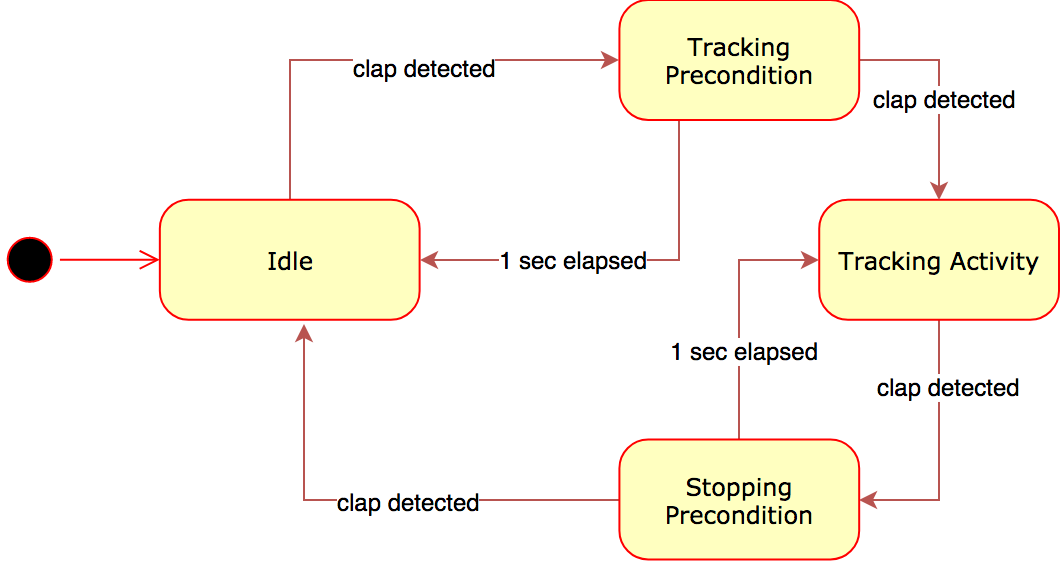
\includegraphics[width=.9\linewidth]{./imgs/statemachine.png}
\end{center}

There are a total of four states in which the app can be in. 
\begin{itemize}
\item Idle: The initial state when starting the app and the state after an activity tracking has been completed.
\item StartPrecondition: If the app is in the idle state and a clap is detected, the state machine switches to this state. When switching to this state, a timer is started which defines the time window in which the second clap must occur in order to switch the state to TrackingActivity. If the timer expires before another clap is detected, the state machine switches back to the idle state.
\item TrackingActivity: After a second clap is detected while the timer of the start precondition has not yet elapsed, the state machine changes to this state and starts capturing the time by saving a time stamp.
\item StoppingPrecondition: If the state machine is in the TrackingActivity state and a clap occurs, then the state machine switches to this state, which behaves in the same way as the StartingPrecondition, except that on a successful second clap, it changes to the idle state and the tracking of the current activity is ended.
\end{itemize}

\subsection{Architecture}
\label{sec:org393d659}

\begin{center}
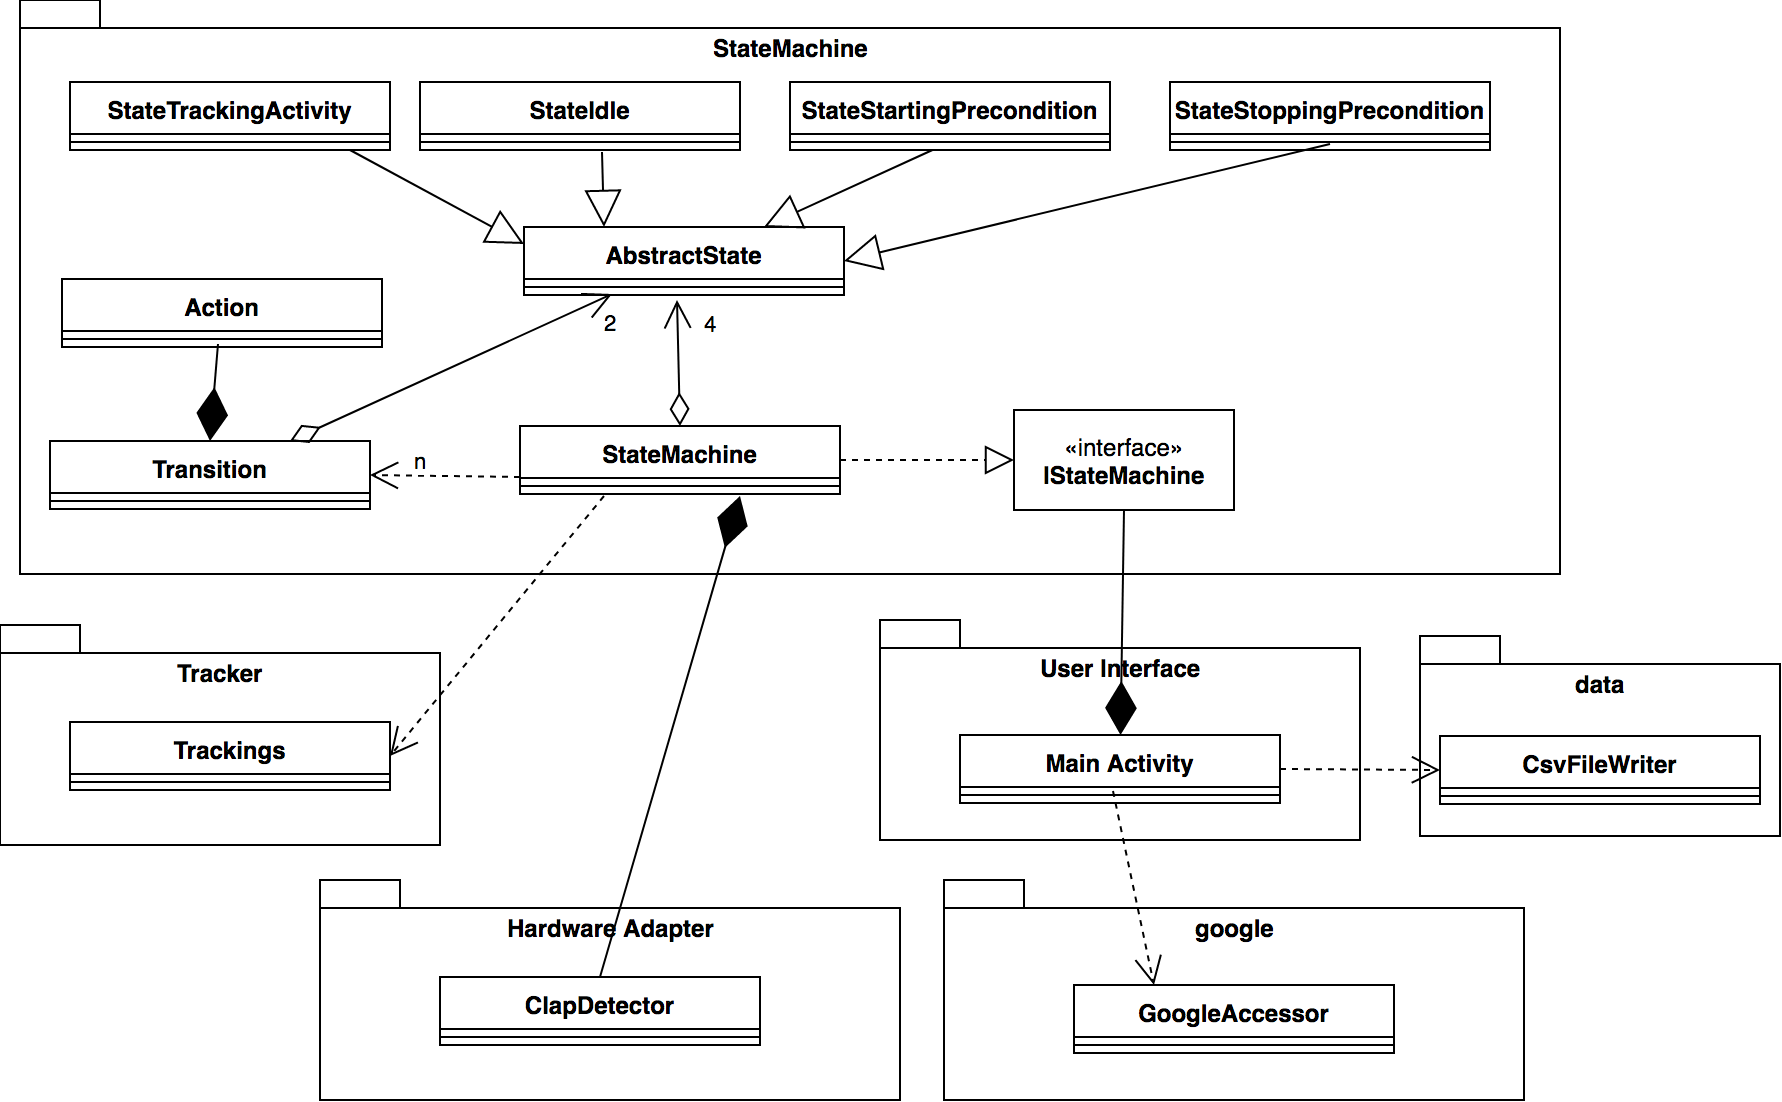
\includegraphics[width=.9\linewidth]{./imgs/classUML.png}
\end{center}

\begin{enumerate}
\item StateMachine
\label{sec:org9ea54c6}

The state machine presented in the previous chapter takes care of the logic 
of the app and switches back and forth between states when registering the corresponding event. 
The Statemachine class is the center of the package of the same name and performs the tasks described in the previous chapter.
It holds instances of all four states and a configuration of all possible transitions between the individual states.
Each transition in the configuration is also linked to an action that determines the event that triggers 
the transition. Each transaction also defines the previous state and the next state.
When a transition is triggered, other operations are also executed that either adapt UI elements to the new 
state or execute other functions that are important for parts of the business logic.

\item Hardware Adapter
\label{sec:org0a1c43f}
The hardware adapter package includes the ClapDetector class, which uses the SmartPhone's microphone to listen 
for ambient sounds and tries to detect a clap from the recorded frequencies. When a clap is detected, 
a handler is triggered in the state machine. This triggers a transition between two states in the state machine.
This is illustrated in figure TODO: REF EINBAUEN !!!!.

\item Tracker
\label{sec:orgd2cdde2}

One of the operations triggered by the investments in the state machine is to start or stop the tracker, 
which stores the activities of the user together with the measured times in a list.

\item User Interface
\label{sec:org2938786}

The User Interface package contains the main activity of the app, which initializes the other functions of 
the program including the state machine. The goal was that the Main Activity class should contain as little 
business logic as possible. The business logic has been implemented almost completely in the state machine. 
If possible, the class should only provide and control the UI elements of the app. It also controls the permissions 
request to the user, which the user must give in order for the apps to work properly.

\item Google
\label{sec:org3d3dca0}
This package contains the GoogleAccessor class, which was initially designed to upload the test data stored on the 
smartphone via the CSVWriter class to the Google Cloud. Once enough data has been collected, this functionality has 
been disabled for the release of the app. The reason for this was that access to the cloud required signed apk, 
which had nothing to do with the pure functionality of the app. Commenting out the code of this feature should 
avoid unnecessary problems when starting the app.

\item Data
\label{sec:orgdeb052b}
The data package contains the CsvFileWriter class, which stores the frequencies recorded by the ClapDetector in 
CSV files on the memory of the smartphone. This functionality was used during development to collect test data 
for later analysis.
\end{enumerate}

\subsection{UI Design}
\label{sec:orgc19d2ea}

\begin{center}
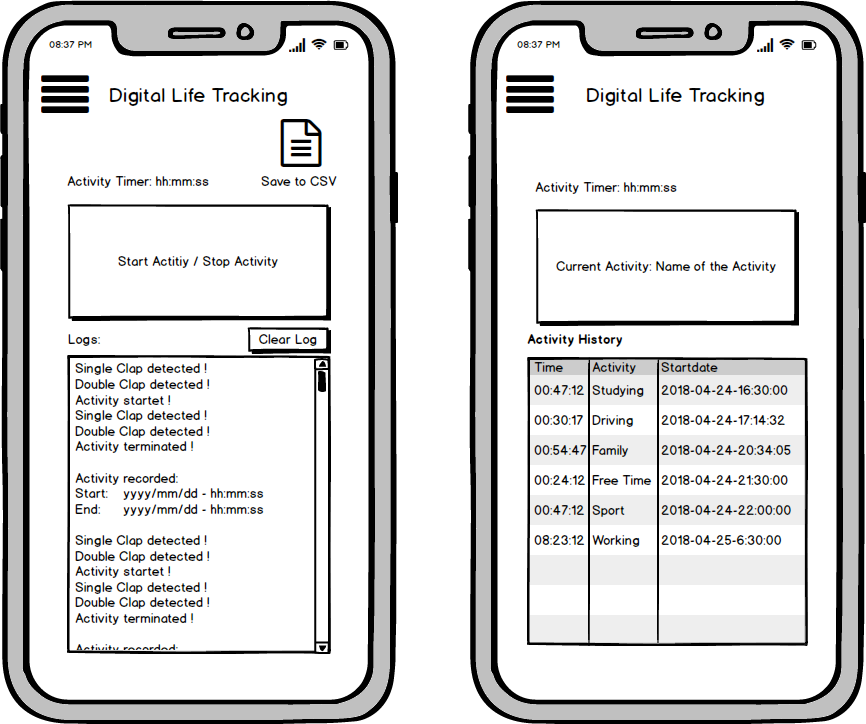
\includegraphics[width=.9\linewidth]{./imgs/mock.png}
\end{center}

\chapter{Conclusion}
\label{sec:org9a10a6c}
\section{Current State}
\label{sec:org4afd87a}
\subsection{Evalutation}
\label{sec:org350e527}
\begin{itemize}
\item How reliable can our implementation detect clap.
\item Benchmark
\begin{itemize}
\item How many time false positives where detected ( 20x husten, 20x schnipsen, 20 klatschen)
\item Show statistics by trying it out (maybe in different environments (loud,
silent rooms, outdoors)
\end{itemize}
\end{itemize}

Refer to to evalution part above. State how difficult this was and the time
needed to try out more advanced solutions (AI) was not enough.

\section{Project Outlook}
\label{sec:orgfa9fd4b}
Maybe add more debug functionallity inside the App, be able to not only tweak
parameters inside the code, but also with UI Controls inside the app.

Whistling detection instead of clapping.







\chapter{Referernces}
\label{sec:orgb5557bc}
\url{http://www.klangfuzzis.de/showthread.php?679817-Was-hat-in-etwa-wie-viel-hz}

\chapter{Aufgaben für uns noch:}
\label{sec:org5420eeb}
\subsection{{\bfseries\sffamily TODO} Tarsos Code rausnkopieren}
\label{sec:org962ce9e}
\subsection{{\bfseries\sffamily TODO} State-machine implement}
\label{sec:org5263181}
\subsection{{\bfseries\sffamily TODO} Fork vom android und unsere repo reinkopieren}
\label{sec:orge187f87}
\end{document}